% BLAST seeding
%
% Basic description of the seeding component of the BLAST algorithm

\subsection{BLAST Seeding}
\begin{frame}
  \frametitle{Word Hits}
  \begin{itemize}
    \item A \emph{word hit} is a short sequence and its \emph{neighbourhood}
    \item \emph{neighbourhood}: words of same length whose aligned score is greater than or equal to a threshold value $T$
    \item Three parameters: scoring matrix, word size $W$, and $T$
  \end{itemize}
  \begin{center}
    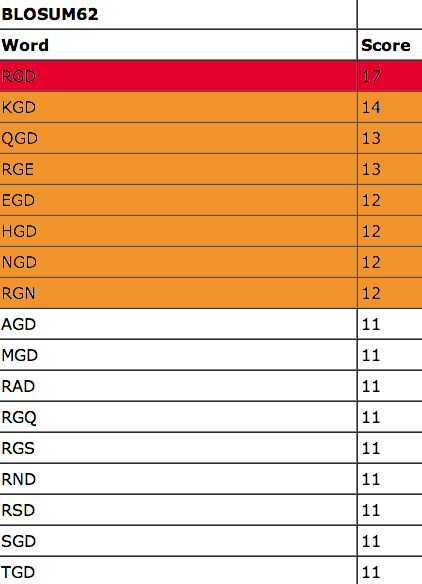
\includegraphics[width=0.3\textwidth]{images/neighbourhood} 
  \end{center}    
\end{frame}

\begin{frame}
  \frametitle{Seeding}
  \begin{itemize}
    \item BLAST assumption: significant alignments have \emph{words} in common
    \item BLAST finds word (\emph{neighbourhood}) hits in the database index
    \item Word hits are used to \textit{seed} alignments
  \end{itemize}
  \begin{center}
    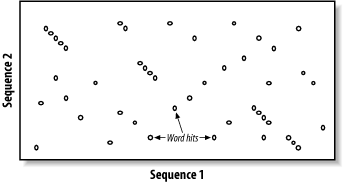
\includegraphics[width=0.5\textwidth]{images/seeding} 
  \end{center}    
\end{frame}

\begin{frame}
  \frametitle{Seeding Controls Sensitivity}
  \begin{itemize}
    \item Word size $W$ controls number of hits (smaller words $\implies$ more hits)
    \item Threshold score $T$ controls number of hits (lower threshold $\implies$ more hits)
    \item Scoring matrix controls which words match
  \end{itemize}
  \begin{center}
    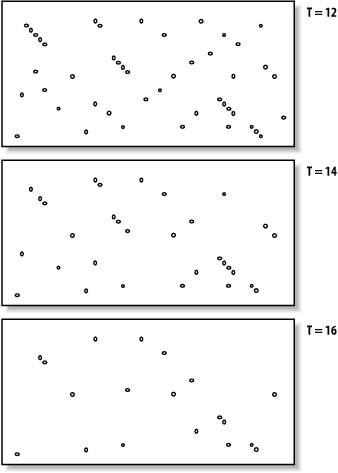
\includegraphics[width=0.25\textwidth]{images/seeding_t} 
  \end{center}    
\end{frame}

\begin{frame}
  \frametitle{The Two-Hit Algorithm}
  \begin{itemize}
    \item BLAST assumption: word hits cluster on the diagonal for significant alignments
    \item The acceptable distance $A$ between words on the diagonal is a parameter of your model
    \item Smaller distances isolate single words, and reduce search space
  \end{itemize}
  \begin{center}
    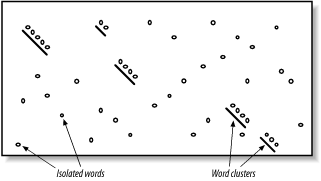
\includegraphics[width=0.5\textwidth]{images/two_hit} 
  \end{center}    
\end{frame}
